\documentclass{sig-alternate}

% some more configurations
%-- Package hyperref ------------------------------------------------------------------------------
\usepackage[
	plainpages=false, %Gibt an auf welcher Seite die pdf-Darstellung beginnt.
	pdfpagelabels,
	pdftex=true,
	breaklinks=true, %/false: Gibt an, ob Links umgebrochen werden duerfen.
	%linktocpage=true/false: im Inhaltsverzeichnis sind nur die Seitenzahlen links, nicht der Text
	colorlinks=true, %/false: Links werden eingefaerbt (Farben werden mit linkcolor, anchorcolor ... festgelegt)
	linkcolor=black, %Farbe des verlinkten Textes, Dokument-interne Links
	citecolor=black, %Farbe des verlinkten Textes, Links zum Literaturverzeichnis
	filecolor=black, %Farbe des verlinkten Textes, Links auf lokale Dateien
	urlcolor=black, %Farbe des verlinkten Textes, externe URLs
	%frenchlinks=true/false: Links werden als smallcaps, anstatt farbig dargestellt.
	menucolor=black
]{hyperref}

\hypersetup{
	pdftitle={GreenSubway},
	pdfauthor={Andreas Jahn, Stephan Sigg},
	pdfsubject={GreenSubway},
	pdfkeywords={GreenSubway},
	%pdfpagelayout={TwoColumnRight}
	%bookmarksnumbered=true,
	%bookmarksopen=true,
	%bookmarksopenlevel=1,
	%pdfpagemode=None % None, UseOutline, UseThumbs, FullScreen
}

\begin{document}
%
% --- Author Metadata here ---
%\conferenceinfo{WOODSTOCK}{'97 El Paso, Texas USA}
%\CopyrightYear{2007} % Allows default copyright year (20XX) to be over-ridden - IF NEED BE.
%\crdata{0-12345-67-8/90/01}  % Allows default copyright data (0-89791-88-6/97/05) to be over-ridden - IF NEED BE.
% --- End of Author Metadata ---

\title{Prediction of passenger density in underground Systems}

\numberofauthors{3} %  in this sample file, there are a *total*
% of EIGHT authors. SIX appear on the 'first-page' (for formatting
% reasons) and the remaining two appear in the \additionalauthors section.
%
\author{
% You can go ahead and credit any number of authors here,
% e.g. one 'row of three' or two rows (consisting of one row of three
% and a second row of one, two or three).
%
% The command \alignauthor (no curly braces needed) should
% precede each author name, affiliation/snail-mail address and
% e-mail address. Additionally, tag each line of
% affiliation/address with \affaddr, and tag the e-mail address with \email.
%
% 1st. author
\alignauthor
Andreas Jahn\\
       \affaddr{Kassel University}\\
       \affaddr{Wilhelmh\"oher Allee 73}\\
       \affaddr{Kassel, Germany}\\
       \email{andreas.jahn@uni-kassel.de}
% 2nd. author
\alignauthor
Stephan Sigg\\
       \affaddr{?Institute?}\\
       \affaddr{?P.O. Box 1212?}\\
       \affaddr{G\"ottingen, Germany}\\
       \email{stephan.sigg@udo.edu}
% 3rd. author
\alignauthor
Klaus David\\
       \affaddr{Kassel University}\\
       \affaddr{Wilhelmh\"oher Allee 73}\\
       \affaddr{Kassel, Germany}\\
       \email{david@uni-kassel.de}
}

% Title
\maketitle

% Abstract
\begin{abstract}

This paper provides a provides a comparison between several prediction accounts in the area of the underground stations.

\end{abstract}

% Introduction
\section{Introduction}
\label{sec:introduction}
Context prediction describes the task of forecasting future evolution of a recorded time-series of contextual stimuli from knowledge on historical data, such as trends, periodicity or typical patters~\cite{4011,5001}.
A number of architectures and algorithms have been proposed for context prediction recently~\cite{4027,2097,Prediction_Eldaw_2013} which could achieve respectable performance on various application domains~\cite{4026,Prediction_Zhang_2013}.
However, in order to make an educated choice from the range of available methods for a particular prediction problem at hand, more and widely adopted datasets are required~\cite{Prediction_Zhang_2012}.
In this paper, we contribute towards this aim by reporting on the SEAM4US dataset which is recorded in a Barcelona Metro station.~\footnote{If you are interested in the dataset, please contact the first author}

Possible use cases for prediction include passenger density prediction, passenger navigation prediction or the prediction for energy efficient operation.
% Underground transportation systems have significant impacts on energy consumption at a regional scale. While the transportation systems, i.e. trains, has observed regarding energy efficiency, the subsystems of metro stations and surroundings, such as ventilation, escalator and lightning are mostly unexplored.
% 
% Although a nominally small percentage of energy can be saved with an efficient management of these subsystems, a large energy saving in absolute terms can be obtained. In other words, a 5\% energy saving in non-traction electricity consumption in one year, is equivalent to the electricity consumed in more than 700 households. 
% 
To investigate on energy efficient subsystems (ventilation, escalator, lightning), the EU funded in the Seventh Framework Programme the project "Sustainable Energy mAnageMent for Underground Stations" (SEAM4US). The SEAM4US project develops  a predictive control architecture, which controls proactively the metro station subsystems, taking current and predicted count of persons within the station into account. The count of persons is provided by an enhanced CCTV system. On the same time the count of persons is the basis for the prediction.
\marginpar{
\begin{figure}
     \begin{center}
     \includegraphics[width=\marginparwidth]{Figures/PdG-L3_entranceExit.jpg}
  \caption{Passeig de Gr\`{a}cia Entrance/Exit Gran Via. \cite{TMB_2014}}
  \label{fig:PdG_entranceExit}
     \end{center}
\end{figure}
}

The remainder of this paper is organized as follows. 
First an overview on the SEAM4US project is given. 
This is followed by a description of the pilot station. 
Subsequently the count of persons extraction is described, followed by a detailed view on the passenger density data. 
Last, our conclusions are drawn.

% Introduce the concept of Anticipatory Sensing here

%Underground transportation systems are big energy consumers and have significant impacts on energy consumptions at a regional scale~\cite{anderson_maximizing_2009}. 
%So far, the optimization of the energy efficiency of transportation equipment, the trains, have been considered. 
%However, although a single train is the largest individual consumer of energy from the overall energy load necessary to run a complete underground system, the investments required for this kind of optimisation are also tremendous. 
%Considering the cost and amount of energy that can potentially be saved in different components of an overall underground metro system, it is suggestive to instead intensify the effort towards other directions.   
%In particular, the optimization of the energy efficiency of the metro stations involves much less investments than the ones that are usually applied to transportation means and equipments. 
%Although only a relatively small percentage can be gained with optimal management of a single metro station compared to optimizing trains, the high number of stations in the underground transportation system in total will yield large energy savings in overall terms. 
%For example, all Barcelona (Spain) metro stations consume 63,1 million kWh annually~\cite{TMB}. 
%A relatively small saving of, for instance, only 5\% in the electricity consumption of a single metro station is equivalent to the electricity consumed in more than 700 households during one year.
%In other words, the management of energy consumption in individual metro stations is a high multiplication factor that boosts each relative small saving at a station level to tremendous savings at a metro network level.
%
%Yet, optimization of the energy efficiency of the metro stations operations, is only minimally exploited.
%Possible directions are the optimized management of stations and surroundings, such as ventilation, vertical transportation and lighting which would have a significant impact on the overall energy consumption.
%Currently, the controller for these systems follow simple time and experience-based coarse schedules. 
%In particular, these systems are optimised for peak times and are therefore operating in an inefficient mode over most part of a day.
%
%A seminal opportunity to optimize the energy efficiency and to realize energy savings is to enable the station to control the surroundings, such as ventilation, vertical transportation and lighting adaptively according to the current situation. 
%For instance, the ventilation-fans of a station could be slowing down when the count of passengers does not necessitate full speed.
%
%In order to achieve such context-aware pro-active behaviour in a metro station, basically three parts are required. 
%\begin{enumerate}
% \item[A:] Sensors that are suited to capture the situation over time accurately
% \item[B:] A controller which is able to calculate the appropriate actions.
% \item[C:] Prediction mechanisms that can anticipate the future evolution of the situation in a metro station
%\end{enumerate}
%An underground metro system features a high number of sensors (A) that can be employed to realise pro-active operation.
%These cover even the tracking of people movement and count which is easily possible via the prominently installed CCTV surveillance systems.
%Recently, also a controller (B) which is adaptive on the basis of various environmental factors, forecasts and passenger occupancy has been developed~\cite{guo_intelligent_2013}.
%The predictive component (C) is necessary since changes applied to the system do not immediately take effect. 
%Staying in the above example with the ventilation-fans, it is sufficient for the controller to be aware of the current count of passengers in order to decrease the fan frequency. 
%However, increasing the fan frequency is more complex. 
%Since the increasing of the fan frequency does not have an immediate effect for the air quality, the fan frequency needs to be increased an appropriate time before the station fills again. 
%It is important to note, that such events can typically occur abruptly in an underground metro system. 
%Examples are, for instance, periodic events such as rush hours or the arrival of connecting trains but also rather spontaneous events like sudden strong rain downfall or simply one of the frequent excursion trips from schools where groups of several hundred people float a station in a short time. 
%
%To guarantee the required air quality on every point in time, the ventilation needs to be controlled in a foreseen manner, that means based on the prospective number of passengers in a station.
%
%This paper presents the approach of Anticipatory Sensing for the prediction of the number of passengers in a station.
%
%Anticipatory Sensing relies on current stimuli from the sensing system, recent historical stimuli that represent trends, typical patterns or periodicity over time and explicit knowledge about relevant events and their corresponding characteristic patterns as depicted in figure~\ref{figureAnticipativeSensingSystem}.
%\begin{figure}
% 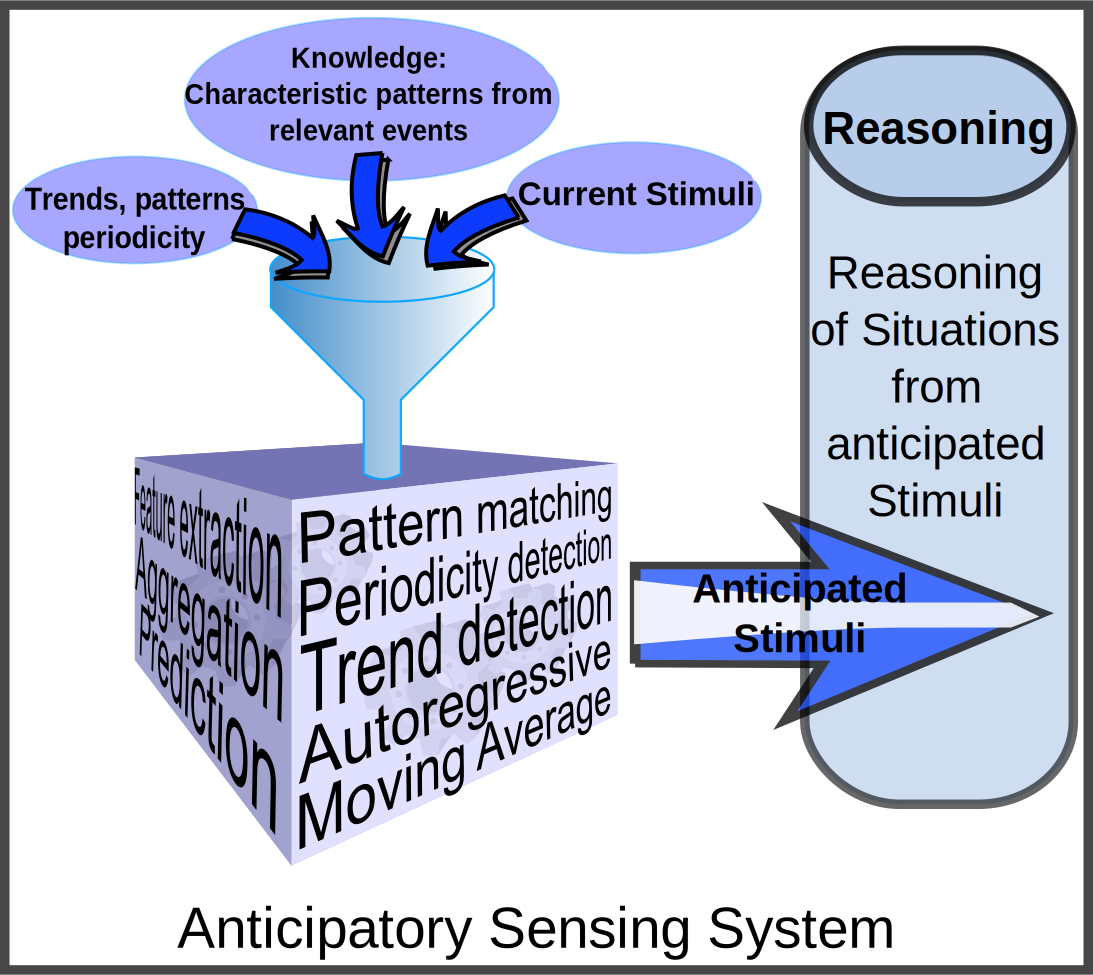
\includegraphics[width=\columnwidth]{Figures/AnticipativeSensingSystem2.pdf}
% \caption{TODO: Improve figure; Schematic illustration of an anticipative sensing system}
% \label{figureAnticipativeSensingSystem}
%\end{figure}
%
%From this information, the series of the current and recent stimuli are analysed for decisive patterns that allow the computation of likely continuation of the observed series of stimuli.
%In particular, in this Anticipatory Sensing step, first, features are extracted from the recent historical time series of stimuli, aggregated and then this series of aggregated features is analysed following multiple approaches from context prediction, pattern matching and time-series forecasting in order to enable a reasoning on possible continuation of this series of stimuli together with their probability.
%
%These anticipated stimuli, which are expected to be observed via the sensing system in the near future are then forwarded to a reasoning component where the anticipated low-level stimuli are classified for situations.
%Note that this order of prediction and reasoning also follows a recent recommendation from~\cite{4027} where the inpact of the order of computations on the prediction accuracy was analysed.
%
%Based on these reasoned situations, the controller of the underground metro system is then in the position to take informed actions, such as, for instance, to increase the fan frequency an appropriate time prior to the actual arrival of the crowd in the station.



% State of the art
\section{State of the art}
\label{sec:stateOfTheArt}

State of the art


% Results
\section{Results}
\label{sec:results}

Results

% Conlusion
\section{Conclusion}
\label{sec:conclusion}

In this paper we have discussed ongoing work in the SEAM4US project. 
In particular, we have discussed peculiarities of the Barcelona underground system under observation.
This has in particular shown that there are plenty of CCTV cameras installed in underground metro systems which are capable to generate enormous amounts of feature data which can be utilized, for instance, for the analysis and prediction of passenger density over time.
In particular, we could observe that, although the magnitude of passenger density fluctuation differs depending on where in the system the corresponding cameras are installed, this fluctuation is highly correlated among the CCTV cameras.
Furthermore, the data shows clear patterns that allow prediction of passenger density over time. 
We have therefore investigated the predictability with an Adaptive Network-based Fuzzy Inference System, which has shown good potential for the prediction in various applications. 
In future work we will investigate the predictability of this data to exploit potential energy savings by controlling electricity and fan-speed more accurately and based on actual load.  
In particular, for energy efficient control of this subway subsystem the SEAM4US project develops a predictive control architecture. 
The control architecture proactively performs energy management tasks based on situations taking place in the future. 


\let\oldtocsubsection=\tocsubsection
% Acknowledgements
\section*{Acknowledgements}
\label{sec:acknowledgements}

This work was partially funded by the EU-FP7 project "Sustainable Energy mAnageMent 4(for) Underground Systems" (SEAM4US, FP7-ICT, EEB-ICT-2011.6.4). The authors would like to acknowledge the contributions of their partners and colleagues.

\marginpar{
\begin{figure}
\begin{center}
    \includegraphics[width=\marginparwidth]{Figures/Figure_PredictionError1.png}
 \caption{Passenger density prediction error utilising an Adaptive Network-based Fuzzy Inference System}
 \label{figurePredictionError}
 \end{center}
\end{figure}
}

% References
%\section*{References}
\label{sec:references}

\bibliography{literaturGreenSubway.bib}
\bibliographystyle{plain} %alpha plain

%\bibliography{references.bib}
%\bibliographystyle{plain} %alpha plain



\end{document}